\documentclass[10pt]{beamer}

\usepackage[english]{babel}
\usepackage[utf8]{inputenc}
\usepackage[T1]{fontenc}
\usepackage{lmodern}

\usepackage{layout}
\usepackage{epsfig}
\usepackage{graphicx}
\graphicspath{{images/}}

\usepackage[squaren, Gray]{SIunits}
\usepackage{sistyle}
\usepackage[autolanguage]{numprint}

\usepackage{amsthm}
\usepackage{amsmath}
\usepackage{amssymb}

\usepackage{mathrsfs}
\usepackage{wrapfig}
\usepackage{url}
\usepackage{multirow}
\usepackage{array}
\usepackage{pgfplots}

\usepackage[version=3]{mhchem}

\usepackage{wasysym}

%Bibtex
%\usepackage[square]{natbib}
%\newcommand{\newblock}{}

\usetheme{Warsaw}

\usepackage{graphicx}
\usepackage{epsfig}
\usepackage{epstopdf}
%\DeclareGraphicsRule{.eps}{pdf}{.pdf}{`epstopdf #1}
%\pdfcompresslevel=9
%\epstopdfsetup{suffix=}
\usepackage{todonotes}
\title{PageRank}
\author{
  Quentin Laurent
  \and
  Benoît Legat
}

\newcommand\si[2]{\numprint[#2]{#1}}

\begin{document}

\begin{frame}
  \maketitle
\end{frame}
\begin{frame}
\tableofcontents
\end{frame}
\section{Introduction to pagerank}
\setbeamertemplate{background canvas}{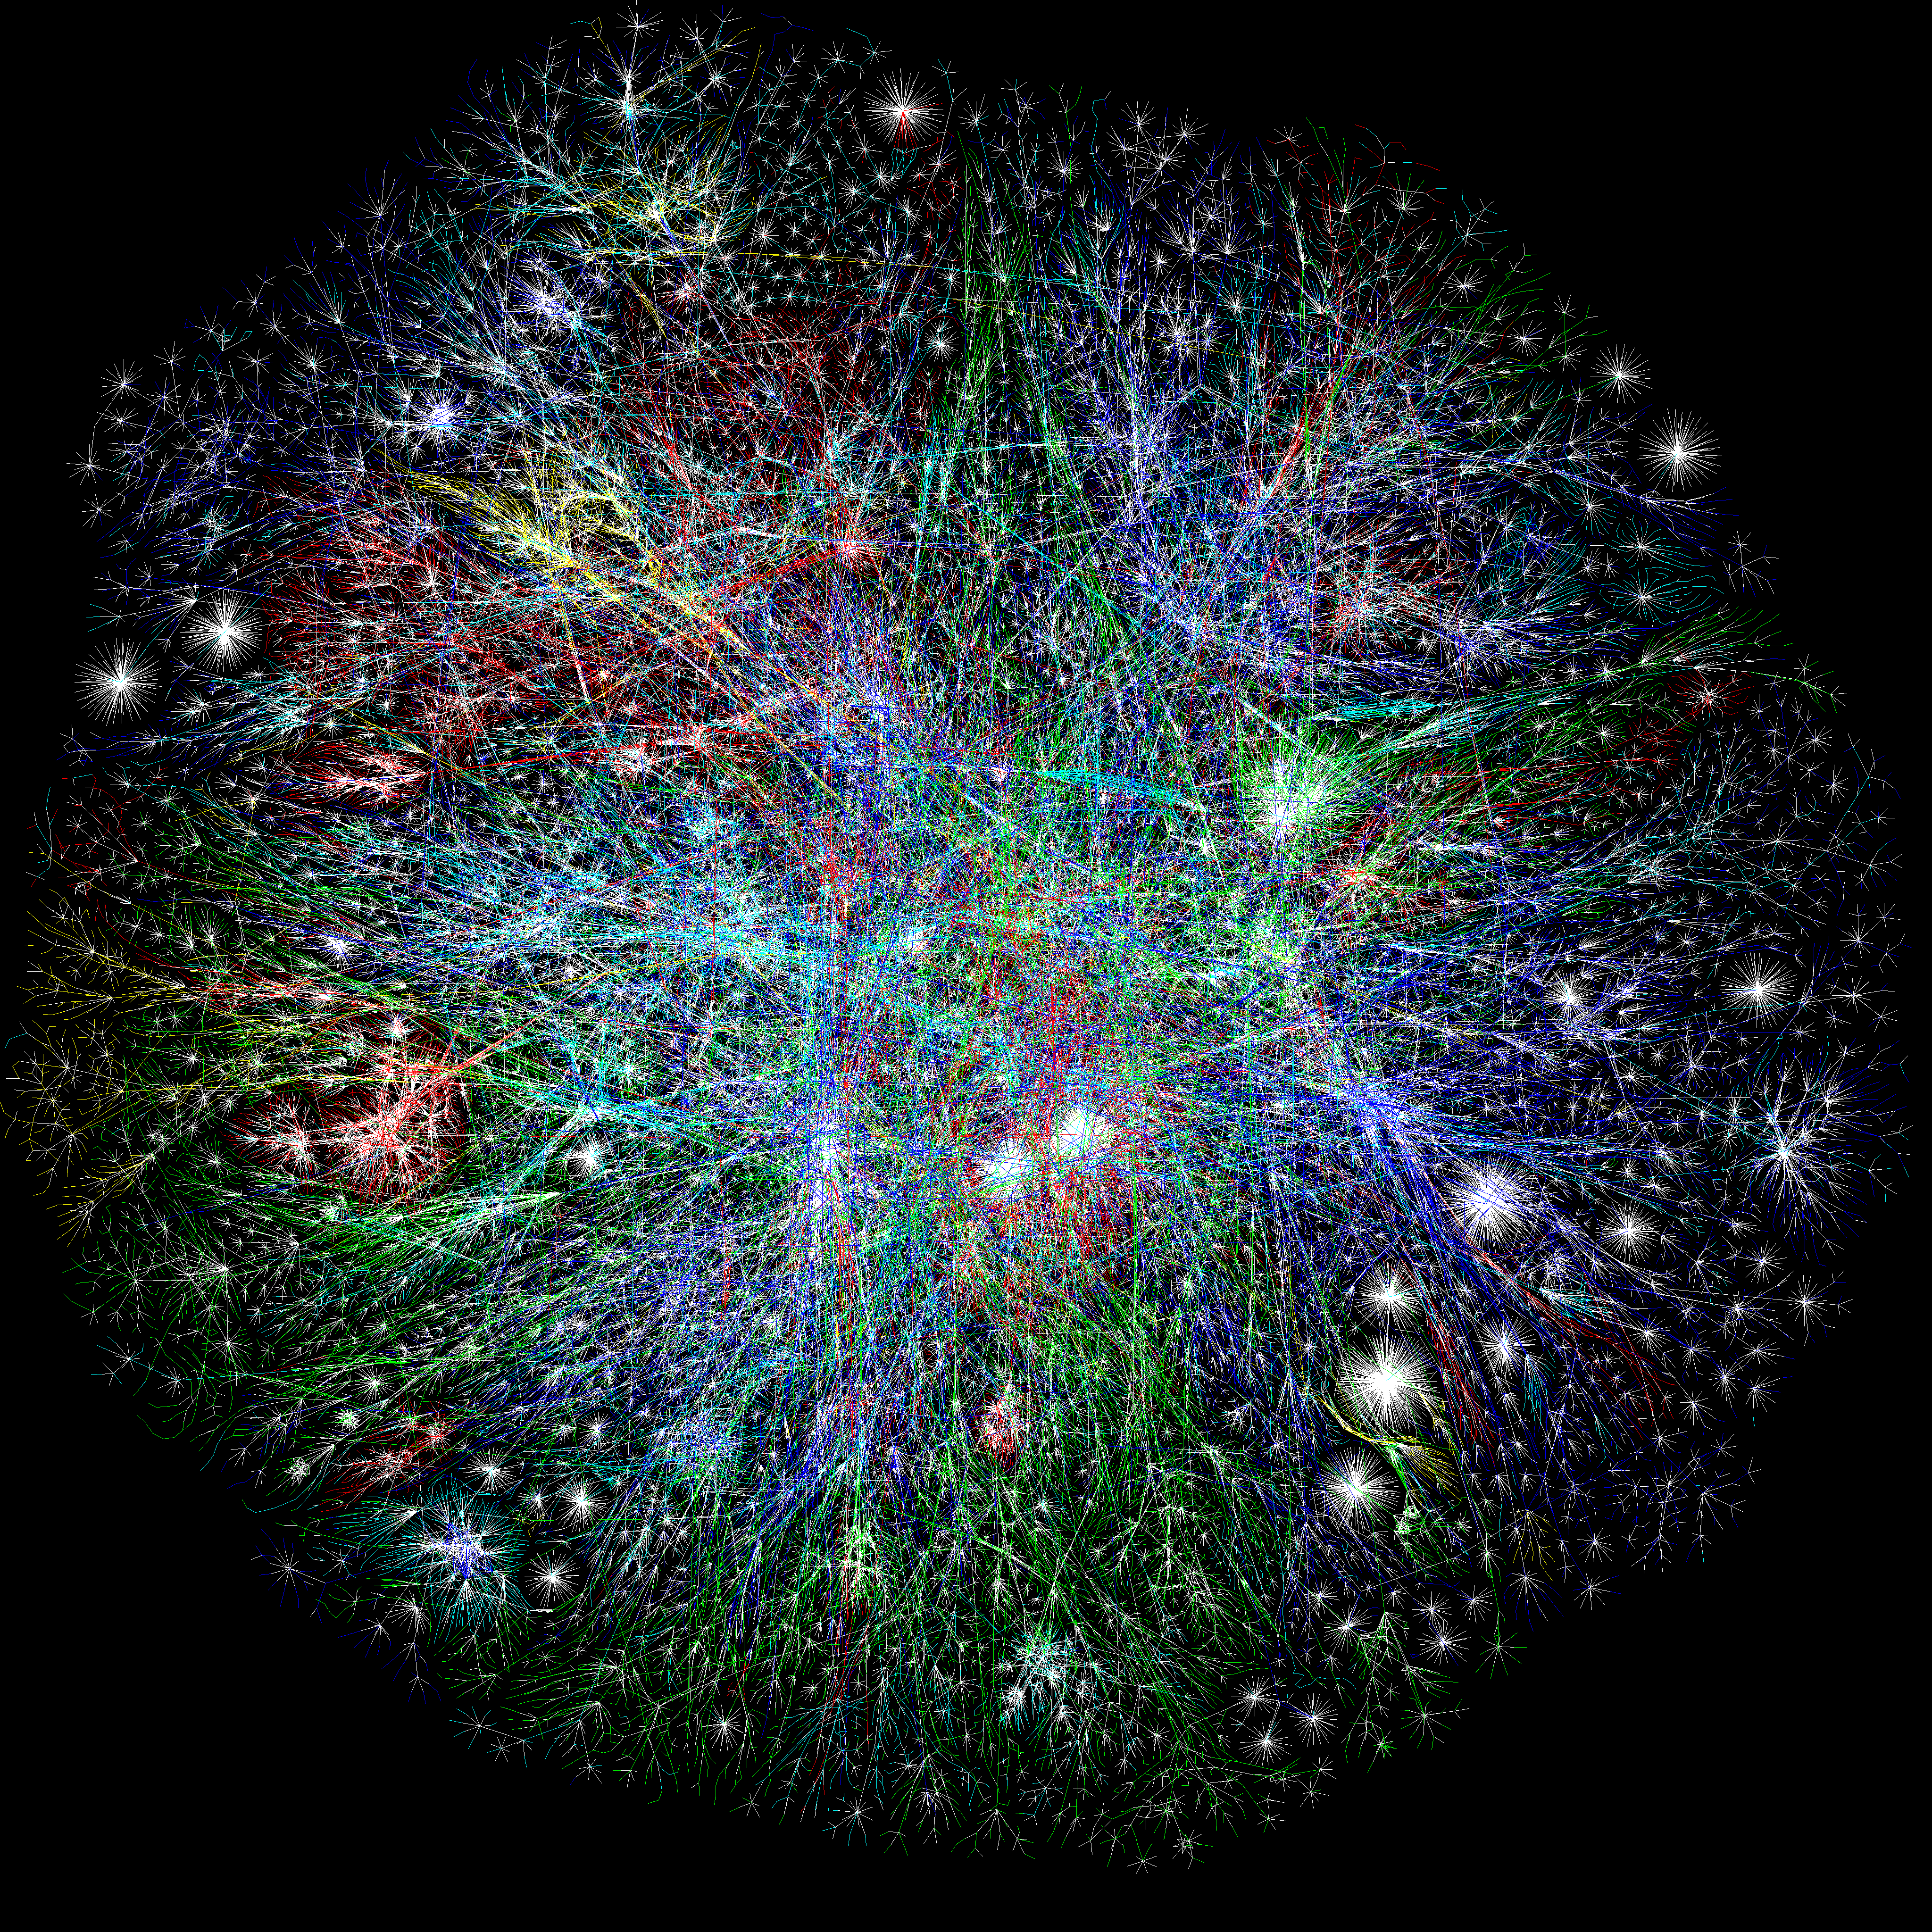
\includegraphics[width = \paperwidth]{InternetGraph.png}}
\setbeamertemplate{blocks}[rounded][shadow=false]
\begin{frame}
\frametitle{Pagerank : motivation}
	\begin{block}{Where to start searching the web}
	How to find one's way through the millions of webpages of the web?
	\end{block}
	%\begin{figure}
%	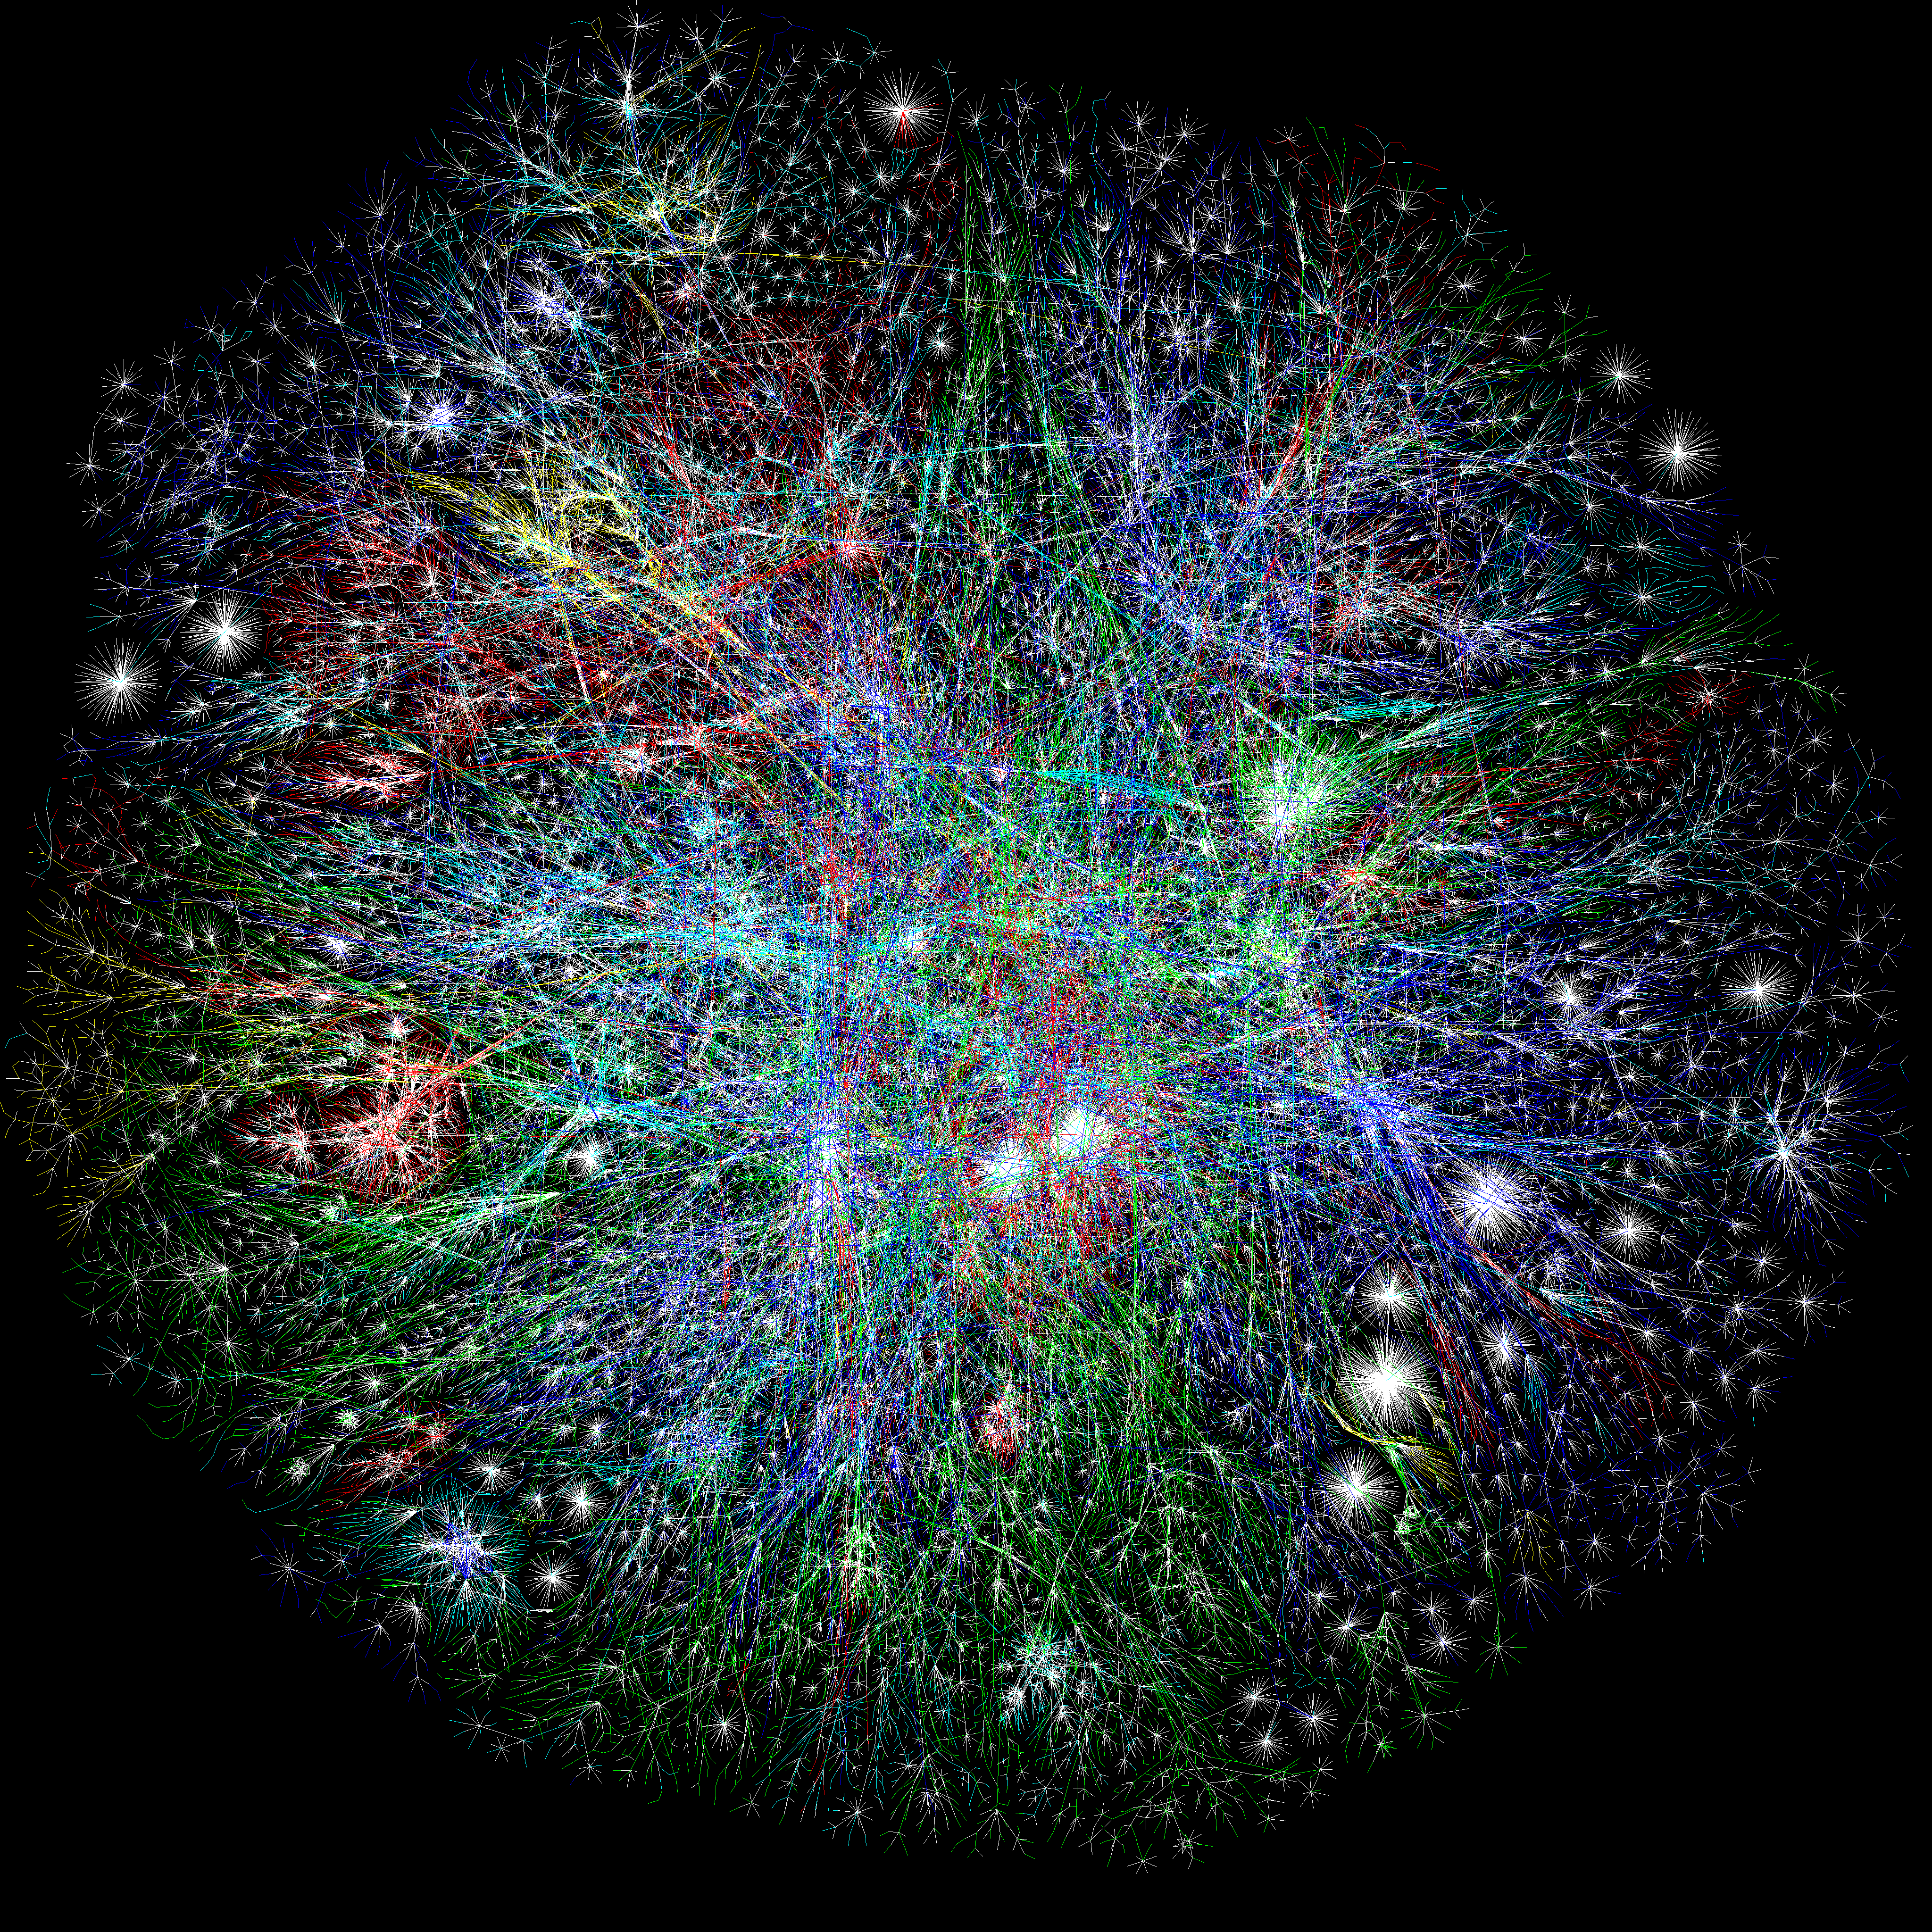
\includegraphics[width = 8cm]{InternetGraph.png}
%	\end{figure}
  % Quentin
\end{frame}
\setbeamertemplate{background canvas}{}
\setbeamertemplate{blocks}[rounded][shadow=false]
\begin{frame}{Search engines}
\begin{block}{Answer}
\begin{itemize}
\item Use of search engines
\item Centralization : you only need to know the address of the search engine
\end{itemize}
\end{block}
\begin{figure}
\centering
	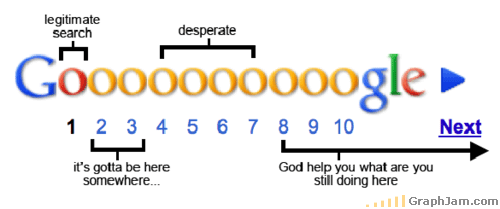
\includegraphics[width = 8cm]{google-search-result-pages.png}
\end{figure}

\end{frame}
\begin{frame}{Early search engines}
\begin{block}{At first}
\begin{itemize}
\item Early search engine's simply listed the terms in each page, making it easy to fool the search engine using \textbf{term spam}

\end{itemize}
\end{block}
\begin{figure}
	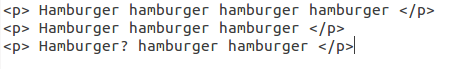
\includegraphics[width = 10cm]{termspam.png}
\end{figure}
\begin{block}{Pagerank}
\begin{itemize}
\item The game changed with Google's arrival and the use of this algorithm in search engines
\end{itemize}
\end{block}
\end{frame}

\setbeamertemplate{background canvas}{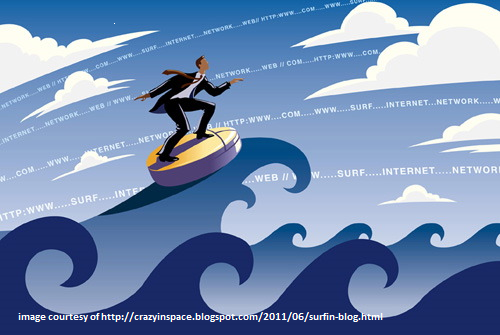
\includegraphics[height = \paperheight]{surfer.png}}
\setbeamertemplate{blocks}[rounded][shadow=false]
\addtobeamertemplate{block begin}{\pgfsetfillopacity{0.7}}{\pgfsetfillopacity{1}}
\begin{frame}{The random web surfer}
\begin{block}{PageRank takes in account}
\begin{itemize}
\item Likelihood of a random surfer to end up on a particular page 
\item Content of a page related to the words used in the link to that page \textit{Todo : Comment on prend ça en compte?}
\end{itemize}
$\rightarrow$ The users of the web vote for the best pages by placing links to useful websites on their own sites\\
$\rightarrow$ Has been proved to work empirically
\end{block}
%\begin{figure}
%	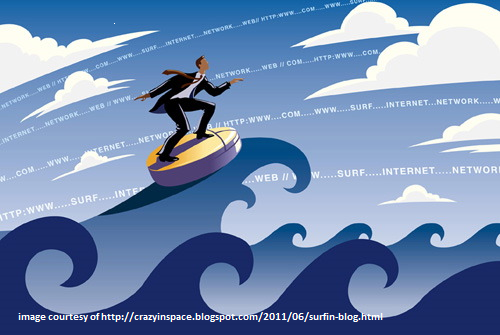
\includegraphics[width = 5cm]{surfer.png}
%\end{figure}
\end{frame}


\setbeamertemplate{background canvas}{}
\setbeamertemplate{blocks}[shadow=true]
\section{Definition of pagerank}
\begin{frame}{Definition of pagerank}
\begin{columns}
\begin{column}{5cm}
\begin{block}{The internet as a graph}
Directed graph $\mathcal{G}$, pages are nodes and there is an arc from p1 to p2 if there is at least one link from p1 to p2
\end{block}
\end{column}
\begin{column}{5cm}
\begin{figure}[r]
	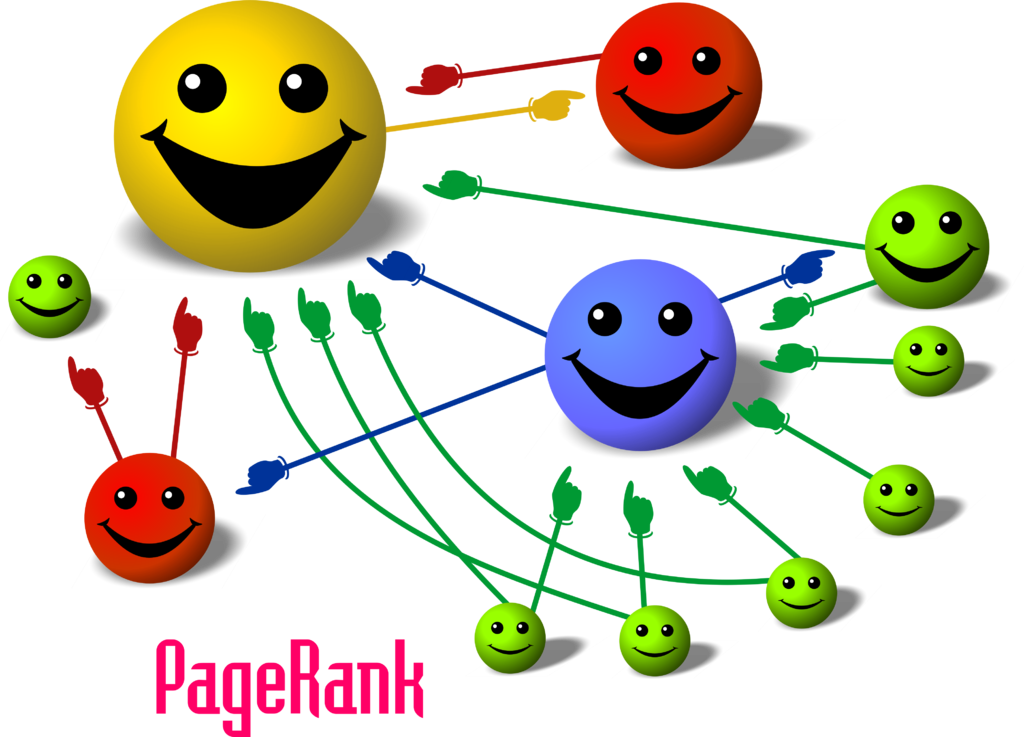
\includegraphics[width =4.5cm]{PageRank-hi-res.png}
\end{figure}
\end{column}
\end{columns}
\begin{definition}
\begin{itemize}
\item A function that assigns a real number to each page
\item It corresponds to the probability of a random surfer of ending up on this particular page after an infinity of steps through the graph
\end{itemize}
$$Pgrk(\mathcal{G}) = v = \begin{vmatrix}v_0\\
				\vdots \\
				v_n\end{vmatrix} $$
\end{definition}

\end{frame}
\begin{frame}{Construction of the transition matrix}
\begin{block}{Transition matrix}
\begin{itemize}
\item Probability of one surfer of going to a linked page is $\frac{1}{l}$ where l is the amount of links leaving that page
\item Henceforth the sum of the elements of each column is always 1 if there is at least one vertex leaving each page
\end{itemize}
\end{block}
\begin{columns}
\begin{column}{\paperwidth/2}
\begin{figure}
	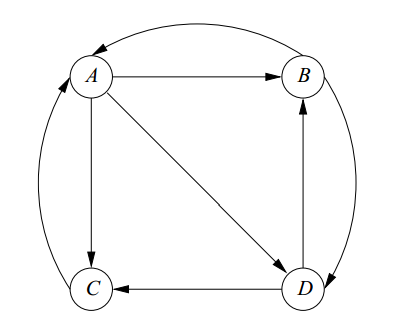
\includegraphics[width = 5cm]{graph1.png}
\end{figure}
\end{column}
\begin{column}{\paperwidth/2}
$$\begin{vmatrix}
0 & \frac{1}{2} & 1 & 0 \\
\frac{1}{3} & 0 & 0 &\frac{1}{2} \\
\frac{1}{3} & \frac{1}{2}&  0& 0 

\end{vmatrix}$$
\end{column}
\end{columns}
\end{frame}
\begin{frame}{Definition of pagerank}
\begin{block}{Probability of distribution for the location of a random surfer}
At first : $$v_0 = \begin{vmatrix}\frac{1}{n}\\
				\vdots \\
				\frac{1}{n}\end{vmatrix}$$
Law of total probability : $P(A) = \sum_n P(A|B_n)P(B_n)$\\
After 1 step, 2 steps, ... v becomes $Mv_0$, $M^2v_0$, ...
\end{block}
\begin{block}{Does it converge?}
We approach a limiting distribution if the graph is strongly connected and there are no dead ends.\\
v = Mv, v is the principal eigenvector \textit{Todo : proof}
For the world wide web : 50-75 iterations are generally needed
\end{block}
\end{frame}
\begin{frame}{Application to search engine}
\begin{itemize}
\item \textbf{Collect the data} Web crawlers
\item \textbf{Selection of pages} A page needs to satisfy certain criteria to be considered in the pagerank, then other properties are used to determine (ex : search terms in prominent places)
\item \textbf{Computation of pagerank} The algorithm described is used to associate a number to each page
\item \textbf{Determination of the order on the result page} Each search engine has a secret formula in which pagerank plays an important role
\end{itemize}
\end{frame}
\begin{frame}{Graph to SCC with DAG}
\end{frame}

\begin{frame}{Actual Web graph}
\end{frame}

\begin{frame}{Dead end ! Are we dead ? Is it the end ?}
\end{frame}

\begin{frame}{Spider traps ! Are we trapped ?}
\end{frame}

\begin{frame}{Topic sensitive}
  % Quentin
  \begin{block}{Biased random walks}
  \begin{itemize}
  \item Same principle as taxation
  \item This time we use a teleport set S relative to a certain topic
  \end{itemize}
  $$ v' = \beta Mv + (1-\beta)e_s/|S|$$
  \end{block}
\end{frame}
\begin{frame}{Deploying topic sensitive PageRank}
\begin{block}{Steps for topic sensitive PageRank}
\begin{itemize}
\item Decide on the topics
\item Pick a teleport set S
\item Relate search queries with a topic(tricky : user chosen, webpages recently searched or bookmarks, facebook,...)
\item Apply pagerank for selected topic(s)
\end{itemize}
\end{block}
\end{frame}
\begin{frame}{Inferring topics from words}

\end{frame}
\begin{frame}{Hubs and Authorities}
\end{frame}
\section{Implementation}
\begin{frame}{Efficient representation of Transition Matrices}
  % Quentin
\begin{itemize}
\item M is sparse, represent it by its non-zero elements
\item For each column : one integer for the out-degree, one integer per non-zero entry
\end{itemize}
\textbf{Todo : Application to topic sensitive}
\end{frame}

\begin{frame}{Use of MapReduce}
\begin{center}v  is too large to fit in main memory \end{center}
\begin{block}{First approach}
\begin{itemize}
\item Separate v and separate M in k stripes
\item Use of k map tasks whose sum is the result of a pagerank iteration
\item The result v' will not fit in main memory either
\end{itemize}
\end{block}
\begin{block}{Second approach : separate M in blocks}
\begin{itemize}
\item Separate v in k parts and M in $k^2$ squares.
\item Use of $k^2$ map tasks, v is transmitted over the network k times
\item Representing a column of blocks takes more space than a stripe but not too much (max 2 times more because of the repetition of the out degree)
\end{itemize}
\end{block}
\end{frame}
\end{document}

% Sources images : 
% Gooooooogle : http://triooti.com/2014/08/23/google-nous-cache-des-informations-dans-les-recherches/
% Web graph : matthewgress.com
% Pagerank : wikipedia